\documentclass[14pt]{extarticle}
\usepackage{amsmath}
\usepackage{amssymb}
\usepackage{graphicx}
\graphicspath{ {../chap09/} }
\usepackage[top=1in, bottom=0.75in, left=0.75in, right=0.75in]{geometry}
\newcommand*{\Scale}[2][4]{\scalebox{#1}{\ensuremath{#2}}}%
\usepackage{hyperref}
\usepackage[most]{tcolorbox}
\definecolor{bg}{RGB}{255,249,227}


\begin{document}

\section*{Math 208 Discussion Outline for 11/12/2020}

\begin{tcolorbox}[enhanced jigsaw,colback=bg,boxrule=0pt,arc=0pt]
	\resizebox{10cm}{!}{
		{Exam 3 on Thursday, 11/19}
	}\\
\footnotesize{
\begin{verbatim}
Who: All students (Tuesday and Thursday)
Time: Regular class time but arrive early
Where: The Wisconsin Room, in the Union. This is not our usual room.
Sec 608           11:00-11:50     Wisconsin Room East
Sec 610           12:00-12:50     Wisconsin Room West
Sec 612           13:00-13:50     Wisconsin Room East

If you are unable to make it, notify me immediately. If you will miss it due to COVID, you 
must make other arrangements BEFORE November 19.

The exam will be 20 problems, each worth 5 points. No notes or books are allowed. A 
non-graphing calculator is permitted. You must show all of your work. Correct answers 
without sufficient work will receive little to no credit. Answer every question to get 
some credit.

Lastly, Professor Schultz posted a review video. The exam will be very close to the review.
\end{verbatim}
}

\end{tcolorbox}


\subsection{Homework and other due dates}
\begin{itemize}

\item Section 9.5, 9.7 due 11/13
\item Section 9.7 due 11/17
\item In class assignment due 11/15 \\\\
\resizebox{12cm}{!}{
	{When is the right time for Christmas music?}
}
\end{itemize}

\subsection{Questions?}

\subsection{Topics}
\begin{itemize}
	\item Limits and limits at infinity (4 questions)
	\item Derivative: the 4-step process (2 questions)
	\item Differentiation properties \textbf{(10 questions)}
	\item Marginal analysis (4 questions)
	\item Starred problems are likely on the take home version. **
\end{itemize}

\subsection{Practice}
\begin{align*}
	&f(x) =
	\begin{cases}
		x^2+1,  & x <2\\
		x-1, & x>2
	\end{cases} \\
	&\lim_{x \to 2^-} f(x)
	&\lim_{x \to 2^+} f(x)	\\
	&\lim_{x \to 2} f(x)
	&f(2)
	\\\\\\
	&\lim_{x\to 2} \frac{x^2-4}{x-2}	&\lim_{x\to -1}\frac{x|x+1|}{x+1}
\end{align*}
\begin{center}
	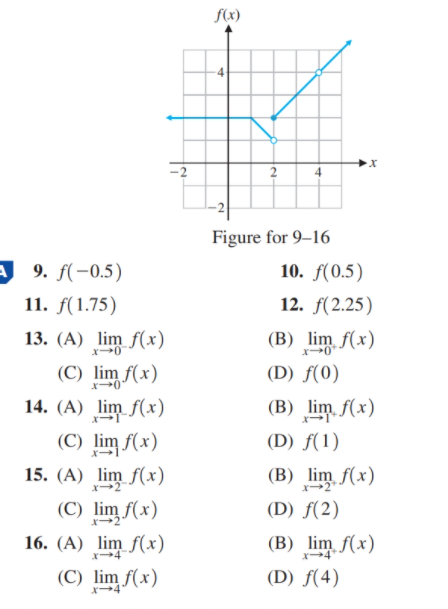
\includegraphics[width=0.65\linewidth]{9-1-9}
\end{center}

\cleardoublepage
For the following, find $\lim_{x\to \infty}f(x):$
\begin{center}
	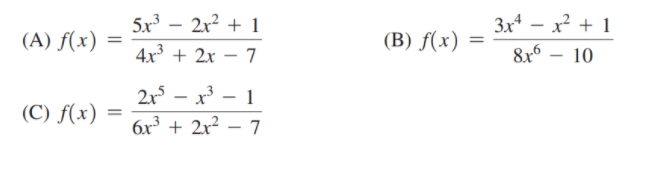
\includegraphics[width=0.85\linewidth]{9-2-11}
\end{center}
Find:
\begin{align*}	
	&\lim_{x \to -\infty}\frac{1}{x}  + x^2 \text{ **}	
	&\lim_{x \to 0^-}\frac{1}{x}  + x^2 \text{ **}
\end{align*}
Use the four step process to find the derivatives:
\begin{align*}
	&f(x) = 4x - x^2
	&f(x) = \frac{1}{x}\\
	&f(x) = \sqrt{x}+2 \text{ **}
\end{align*}
\\
Use rules to find the derivatives of the following:
\begin{align*}
	&g(x)= \frac{30 + x^2 - x^3}{x^2}
	&y = 2 + 5t - 8t^3
	\\\\
	&h(w) = \frac{3w^2}{2} - \frac{7}{5\sqrt[3]{w}}
	&p=(x+1)^2 - x^3 +1
	\\\\
	&w(x) = \frac{3}{2x^2} - \frac{1}{\sqrt[5]{x^3}}
	&y=2x^4(x+1) - x^{-3} +291
\end{align*}
Find the tangent line at $x=4$, where $g(x)$ is:
\begin{align*}
	g(x) = 4\sqrt{x} + 2x^2 +10
\end{align*}

\cleardoublepage

\begin{tcolorbox}[enhanced jigsaw,colback=bg,boxrule=0pt,arc=0pt]
	\textbf{Cost, Revenue, and Profit}
	\begin{align*}
		price(x)& \text{ usually given} \tag{price} \\
		R(x)&= x* price(x) \tag{revenue} \\
		C(x)& \text{ usually given} \tag{cost} \\
		P(x)&= R(x) - C(x)\tag{profit}
	\end{align*}
\end{tcolorbox}
\begin{tcolorbox}[enhanced jigsaw,colback=bg,boxrule=0pt,arc=0pt]
	\textbf{Exact Cost, Revenue, and Profit}
	\begin{align*}
		\text{exact cost} &= C(x+1)-C(x) \\
		\text{exact revenue} &= R(x+1) - R(x) \\
		\text{exact profit} &= P(x+1) - P(x)
	\end{align*}
\end{tcolorbox}


\begin{center}
	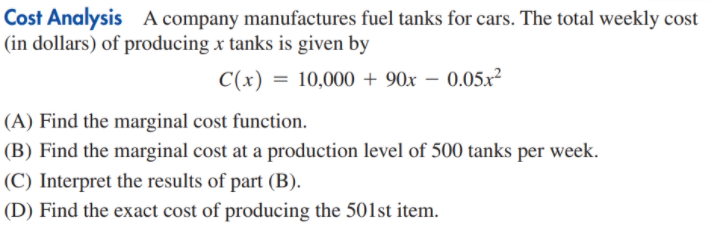
\includegraphics[width=1\linewidth]{9-7-7}
\end{center}
(E) Find the marginal cost approximation of producing the 501st item.
\\
\\
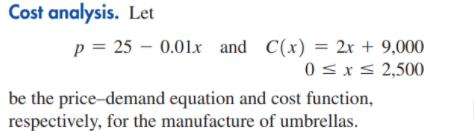
\includegraphics[width=0.75\linewidth]{9-r-1}
\\
(A) Find the marginal cost\\
(B) Find the revenue function and find the marginal revenue.\\
(C) Find the profit and marginal profit\\
(D) Evaluate the marginal profit at $x=1000, 1150, 1400$.

\cleardoublepage






\end{document}
